%\documentclass[10pt, conference, compsocconf, draft, onecolumn]{IEEEtran}

\documentclass[10pt, conference, compsocconf]{IEEEtran}

\IEEEoverridecommandlockouts

\usepackage{balance}
\usepackage{graphicx}
\usepackage{url}
\usepackage{xcolor}
\usepackage{multirow}
\usepackage{epsfig}

%\usepackage{lineno}

\usepackage[dvips]{hyperref}
\usepackage{cite}

\hypersetup{
  bookmarks = false,
  pagebackref=true,
  pdftoolbar=true,
  pdfnewwindow=true,
  pdfmenubar=true,
  pdftitle = {A Novel Anti-Forensics Technique for the Android OS},
  pdfkeywords = {Digital Forensics; Mobile Forensics; Anti-Forensics; Mobile Anti-Forensics; Counter-Forensics; Android OS; Android Forensics; Android Anti-Forensics; Flash Memory; NAND; Secure Deletion; Sanitization.},
  pdfauthor = {Pietro Albano, Aniello Castiglione, Giuseppe Cattaneo and Alfredo De Santis},
  pdfsubject =  {Sixth International Conference on Broadband and Wireless Computing, Communication and Applications  - BWCCA-2011},
  pdfcreator =  {Dr. Aniello Castiglione - castiglione@ieee.org},
}

\begin{document}

\title{A Novel Anti-Forensics Technique\\ for the Android OS}


\author{
\IEEEauthorblockN{Pietro Albano\IEEEauthorrefmark{1}, Aniello Castiglione\IEEEauthorrefmark{2}\thanks{Corresponding author: Aniello Castiglione,~Member,~\textit{IEEE},~\href{mailto:castiglione@ieee.org}{castiglione@ieee.org},~Phone: +39089969594,~FAX: +39089969821}, Giuseppe Cattaneo\IEEEauthorrefmark{4}, Alfredo De Santis\IEEEauthorrefmark{3}}

\IEEEauthorblockA{Dipartimento di Informatica ``R.M. Capocelli''\\
Universit\`{a} degli Studi di Salerno\\
%Via Ponte don Melillo,\\
I-84084 Fisciano (SA), Italy\\
\href{mailto:pietro.albano@gmail.com}{pietro.albano@gmail.com}\IEEEauthorrefmark{1},  \href{mailto:castiglione@ieee.org}{castiglione@ieee.org}\IEEEauthorrefmark{2},
\href{mailto:cattaneo@dia.unisa.it}{cattaneo@dia.unisa.it}\IEEEauthorrefmark{4},  \href{mailto:ads@dia.unisa.it}{ads@dia.unisa.it}\IEEEauthorrefmark{3}}

}

\maketitle

%\linenumbers

\begin{abstract}
In recent years traditional mobile-phones, used only to make calls and send text messages, have evolved into even more versatile and powerful devices (smartphones, tablets, etc.). These devices use a NAND flash memory type to store data, due to it being a memory that has been optimized for the fast updating of data. These flash memory drives usually contain sensitive data that could be a possible danger to the user's privacy.

This paper proposes a new anti-forensics technique for mobile devices with the Android OS. The technique makes it possible to modify and erase, securely and selectively, the digital evidence on an Android device without having to use any cryptographic primitives or make any file system changes. While the use of cryptographic primitives or changes to the file system create considerable suspicion in a forensic analysis, the proposed technique uses simple software tools commonly used in *nix-like OSes such as the Android OS.
\end{abstract}

\begin{IEEEkeywords}
Digital Forensics; Mobile Forensics; Anti-Forensics; Mobile Anti-Forensics; Counter-Forensics; Android OS; Android Forensics; Android Anti-Forensics; Flash Memory; NAND; Secure Deletion; Sanitization.
\end{IEEEkeywords}

\section{Introduction}

Gartner claimed~\cite{Gartner} that in 2011 468 million mobile devices would be sold, i.e. 57.7\% more than last year. In addition, according to the same research agency, in 2012 there will be 632 million smartphones in the world and in 2015, 1.1 billion. In 2012, half (49.2\%) of the 632 million smartphones in circulation will work on the Android OS.

%%%    Nel 2011, ha sottolineato Gartner~\cite{Gartner}, dovrebbero essere venduti 468 milioni di dispositivi mobile, vale a dire il 57.7\% in pi\`{u} rispetto allo scorso anno. Sempre secondo la societ\`{a} di ricerche, nel 2012 saranno 632 milioni di SmartPhone nel mondo e nel 2015 saranno 1.1 miliardi.
%%%    Nel 2012 met\`{a} (49.2\%) dei 632 milioni di SmartPhone in circolazione avranno cuore Android.

The data stored in a smartphone can be a threat to the user's privacy. It is worth recalling that a classic mobile phone contains a large amount of private information (contacts, text messages, call lists). Additional sensitive information stored on smartphones includes emails, websites visited, chat messages, geo-location information, etc.. All this information can give a well-defined profile of its user in order to reconstruct his actions at a specific time. An individual who wants to protect his privacy, and in particular delete or modify in a secure and selective way any digital evidence stored on his smartphone, can use anti-forensics techniques.

%%%    I dati presenti in uno SmartPhone possono rivelarsi una minaccia alla privacy degli individui. Basti pensare che un classico cellulare racchiude al suo interno un gran numero di informazioni private (contatti, SMS, lista delle chiamate). Altre informazioni sensibili contenute negli SmartPhone sono e-mail, cronologia dei siti web visitati, messaggi scambiati in chat, informazioni di geolocalizzazione, etc. Queste informazioni, sommate a quelle precedentemente citate, permettono di individuare un profilo ben definito del suo possessore e di ricostruire le sue azioni in un preciso spazio temporale. Un'individuo che vuole difendere la propria privacy ed in particolare cancellare o modificare in maniera sicura e selettiva delle digital evidence presenti sul prorpio SmartPhone pu\`{o} utilizzare tecniche anti-forensics. 
    
A definition of Anti-Forensics, according to~\cite{RH}, is \emph{``...we will consider anti-forensics to be any attempts to compromise the availability or usefulness of evidence to the forensics process. Compromising evidence availability includes any attempts to prevent evidence from existing, hiding existing evidence or otherwise manipulating evidence to ensure that it is no longer within reach of the investigator. Usefulness maybe compromised by obliterating the evidence itself or by destroying its integrity.''}.

While there are currently no papers dealing with the problem of secure modification in flash memories (to the best of the authors' knowledge), few studies have recently proposed techniques for the secure erasing of NAND flash memory drives that are commonly used in smartphones.
%%%    While no paper has addressed the problem of secure modification in flash memories (to the best of author's knowledge), recently alcuni lavori hanno proposto tecniche di cancellazione sicura per le flash memory NAND che sono di comune utilizzo negli SmartPhone.
%%%%Flash memory drives (NANDs) differ from hard drives in both the technology used to store data (flash chips vs. magnetic disks) as well as the algorithms used to manage and access the data. NANDs maintain a layer of indirection between the logical block addresses that computer systems use to access data and the raw flash addresses that identify physical storage. The layer of indirection enhances NAND performance and reliability by hiding the idiosyncratic interface of the flash memory and managing its limited lifetime. However, it can also produce copies of the data that are invisible to the user but that a smart attacker can recover. 
NANDs are different from hard drives and it is uncertain whether techniques and commands developed for hard drives (for example the one presented in~\cite{assd}) will be effective on NANDs.

%%%%The differences between NANDs and hard drives make it uncertain whether techniques and commands developed for hard drives will be effective on NANDs.

%%%Flash memory drives (NANDs) differ from hard drives in both the technology they use to store data (flash chips vs. magnetic disks) and the algorithms they use to manage and access that data. NANDs maintain a layer of indirection between the logical block addresses that computer systems use to access data and the raw flash addresses that identify physical storage. The layer of indirection enhances NAND performance and reliability by hiding flash memory's idiosyncratic interface and managing its limited lifetime, but it can also produce copies of the data that are invisible to the user but that a smart attacker can recover. The differences between NANDs and hard drives make it uncertain whether techniques and commands developed for hard drives willl be effective on NANDs.

In~\cite{FlashMemoryDeletion} and~\cite{NANDSecureDeletion}, all the data is encrypted and each file has its own encryption key which is stored in the header of the file. When wanting to delete a single file, simply delete or overwrite the header. Encrypting the file system or modifying it in order to apply anti-forensics techniques creates a great deal of suspicion during a forensic analysis.

%%%In~\cite{FlashMemoryDeletion} ed in~\cite{NANDSecureDeletion} tutti i dati vengono cifrati, ogni file possiede la propria chiave di cifratura la quale \`{e} memorizzata nell'header del file stesso. Quando si vuole cancellare un singolo file basta cancellare o sovrascrivere il suo header. Cifrare il file system o modificarlo per applicare tecniche anti-forensics, desta non pochi sospetti in una analisi forense.

In~\cite{DGP10}, exploiting a security feature of Android, it is possible that digital evidence is hidden in a private folder which is inaccessible to third-party applications. The private folder is a private directory, created when an application is installed, in which it is possible to save any file type (e.g., text files, multimedia files).
According to~\cite{DGP10}, when a given Android application is uninstalled, the entire set of the related information, including data files and directories, is logically deleted from the file system.

%%%%In~\cite{DGP10}, sfruttando una security feature di Android, possibili digital evidence vengono nascoste in \emph{private folder} inaccessibili da applicazioni di terze parti. Le private folder sono directory private, create nel momento in cui viene installata un'applicazione, all'interno delle quali \`{e} possibile salvare qualsiasi tipo di file (e.g., file di testo, file multimediali). According to~\cite{DGP10} when a given common Android application is uninstalled, the entire set of the related information, including data files and directories, is logically deleted from the File System.
%    Tale metodo \`{e} stato esaminato e sperimentato su diversi dispositivi Android, riscontrando, al momento della disinstallazione, una cancellazione fisica di tutti i file contenuti nel private folder.

This paper introduces a new anti-forensics technique for mobile devices running the Android OS that makes it possible to edit and delete, securely and selectively, the digital evidence generated by the Android OS by using simple software tools, without making changes to the file system or using any cryptographic primitives.\\

%%In questo articolo viene introdotta una nuova tecnica Anti-Foresics per dispositivi mobile con Sistema Operativo Android che permette di modificare e cancellare, in modo sicuro e selettivo, le digital evidence generate dal Sistema Operativo Android utilizzando semplici tool software, senza apportare modifiche al file system e senza l'uso di primitive crittografiche.

The paper is organized as follows: Section~\ref{AndroidOS} briefly describes the Android OS, paying particular attention to the type of file system generally adopted by Android devices as well as the storage device (NAND) generally used. Section~\ref{AndroidForensics} contains the main forensic techniques used on Android devices. Section~\ref{AndroidAntiForensics} describes the proposed anti-forensics technique, while Section~\ref{CaseStudy} describes the technique that have been designed, implemented and tested on a specific Android device. The conclusions are made in Section~\ref{Conclusions}.

%%%%The paper is organized as follows: la sezione~\ref{AndroidOS} fornisce una breve descrizione dell'OS Android, con particolare attenzione al tipo di File System adottato generalmente dai dispositivi Android ed ai supporti di memorizzazione (NAND) presenti in questi ultimi. Section~\ref{AndroidForensics} illustra le principali tecniche forensi utilizzate su dispositivi Android. La sezione~\ref{AndroidAntiForensics} illustra la tecnica anti-forensics proposta; mentre la sezione~\ref{CaseStudy} describes the instances, to Android devices, of such techniques that have been designed, implemented and tested. L'articolo termina con le conclusioni (sezione~\ref{Conclusions}).

\section{The Android OS}\label{AndroidOS}
Android is a set of open-source software elements specif- ically designed and developed by Google for mobile devices. Although it has been designed and developed for mobile devices (e.g., smartphones, tablets, etc.), it includes the OS, a middleware and a set of applications.

%%%%    Android is a set of open-source software elements specifically designed for mobile devices developed by Google. It includes the Operating System, a middleware and a set of applications. Although it has been designed and developed for mobile devices (e.g., Smartphones, Tablet, etc.).

\subsection{The Android File System}\label{AndroidFS}
The vast majority of mobile devices running the Android OS uses, and supports, the YAFFS (Yet Another Flash File System) file system, developed in 2002 and specifically to be used on NAND flash memories. It is also completely open-source. To the authors' knowledge, YAFFS is the only file system type which fully supports flash memory technology~\cite{YAFFSsite}.
%%%%
%%%%The vast majority of mobile devices running the Android OS uses, and natively supports, the YAFFS (Yet Another Flash File System) file system, developed in 2002 specifically to be used on NAND flash memories and being completely open-source. To the authors knowledge, the YAFFS is the only file system type which fully support the flash memory technology\cite{YAFFSsite}

%        La maggior parte dei dispositivi mobili Android utilizza e supporta nativamente il file system YAFFS  sviluppato nel 2002 appositamente per le memorie flash NAND e completamente open-source.
%        YAFFS (Yet Another Flash File System) \`{e} l'unico file system progettato per supportare a pieno le memorie flash~.
YAFFS has several interesting features such as journaling, error correction and verification techniques, which are very useful when dealing with hardware failures/problems that are intrinsic to the flash memory technology. The Android OS is based on the Linux kernel v2.6 and, thanks to it, allows for the distribution of its file system on different storage devices, on both the internal flash memory as well as a microSD that can be inserted into the mobile device.
%%%%
%%%%YAFFS has several interesting features such as \emph{journaling}, \emph{error correction} and \emph{verification} techniques very useful to deal with hardware failures/problems intrinsic to the flash memory technology.
%%%%The Android OS is based on the Linux kernel v2.6 and, thanks to it, allows the distribution of its file system on different storage device, both internal flash memory and on the microSD that can be inserted in the mobile device.
Table~\ref{tab:FSTabNexusOne} describes the structure and organization of the file system present on the mobile device adopted for the case study. The organization of the partitions as well as the mount points shown in Table~\ref{tab:FSTabNexusOne} may change according to different devices. In the column named ``Partition'', the storage device and the partitions of the internal flash memory as well as the microSD are listed. 
%%%%
%%%%In Table~\ref{tab:FSTabNexusOne} is described the structure and the organization of the file system present on the mobile device adopted for the case study. The organization of the partitions as well as the mount points shown in~\ref{tab:FSTabNexusOne} may change on different devices. In the column named ``Partition'' are listed the storage device and the partitions of the internal flash memory and of the microSD. 
The partitions host different data: \verb"mtd0" contains miscellaneous data, \verb"mtd1" the recovery image, \verb"mtd2" the boot partition, \verb"mtd3" the system files, \verb"mtd4" the system cache and \verb"mtd5" the user data. The ``Mount Point'' column lists only those  partitions which are  accessible from the file system, in other words, only the partitions that can be mounted on a branch of the file system. The  last column of Table~\ref{tab:FSTabNexusOne} shows whether the partition is present on the ``Internal'' flash memory or the ``External'' microSD. The most interesting partitions to be considered during a digital forensics analysis are the \verb"mtd3" and \verb"mtd5"  which contain, respectively, the core of the OS and the work space of the user.

%%%%The partitions host different data: \verb"mtd0" contains miscellaneous data, \verb"mtd1" the \emph{recovery image}, \verb"mtd2" the boot partition, \verb"mtd3" the system files, \verb"mtd4" the system cache and \verb"mtd5" the user data. The ``Mount Point'' column lists only those partitions which are accessible from the file system, in other words, only the partitions that can be mounted on a branch of the file system.
%%%%The last column of Table~\ref{tab:FSTabNexusOne} tells whether the partition is present on the ``Internal'' flash memory or on the ``External'' microSD. 
%%%%The most interesting partitions that are interesting to be considered during a digital forensics analysis are the \verb"mtd3" and the \verb"mtd5" which contains respectively the core of the OS and the work space of the user.
%        YAFFS offre feature quali \emph{journaling}, tecniche di \emph{error correction} e \emph{verification} per ovviare ai problemi hardware intrinsici alle flash memory.
%
%        Android \`{e} un SO basato su kernel Linux 2.6 e come tale esso permette di distribuire il propio file system su diversi device, o partizioni presenti su un supporto di archiviazione di massa (flash memory interna o microSD).
%
%%%        In Table~\ref{tab:FSTabNexusOne} viene descritta la struttura e l'organizzazione del file system Android presente sul dispositivo utilizzato nel caso di studio. L'organizzazione delle partizioni e dei mount point descritte in Table~\ref{tab:FSTabNexusOne} varia da dispositivo a dispositivo. In the Partitions column, device or partition on the internal flash memory and on the microSD are listed. In the last column Internal means partition on the internal flash memory while External means partition on the microSD. In the Mount Point column only directories accessible from the file system are listed.
        
%        Nella colonna Partition, ritroviamo i device ovvero le partizioni presenti sulla flash memory interna e sulla microSD (nell'ultima colonna con il termine Internal vengono indicate le partizioni su flash memory interna mentre con External si indicano le partizioni presenti su microSD). La colonna Mount Point elenca le directory attualmente accessibili al file system.
%%%        The partitions contains different data as follows: \verb"mtd0" contains miscellaneous data, \verb"mtd1" the recovery image, \verb"mtd2" the boot partition, \verb"mtd3" the system files, \verb"mtd4" the system cache and \verb"mtd5" the user data.
%%%
%%%        Le partizioni che meritano particolare attenzione, durante un'analisi forense, sono la \verb"mtd3" e la \verb"mtd5" che racchiudono, rispettivamente, il cuore del SO ed il \emph{work space} dell'utente.

The partition \verb"mmcblk0p1", usually formatted with the FAT file system type,  represents the external memory of the mobile device, with it being managed by the user. The partition \verb"mmcblk0p2", which is formatted with the EXT3/EXT4 file system type, starting from Android v2.2 is used as an extension of the internal memory of the mobile device. This partition can only be accessed by the OS and the \emph{root} user.

%%%%The partition \verb"mmcblk0p1" usually formatted with the FAT file system type, represents the external memory of the mobile device and it left to the user wishes. The partition \verb"mmcblk0p2", which is formatted with the EXT3/EXT4 file system type, starting from Android v2.2 is used as an extension of the internal memory of the mobile device. Such partition is accessible only by the OS and by the \emph{root} user.

%%%La partizione \verb"mmcblk0p1", con file system FAT, rappresenta la memoria esterna del dispositivo mobile accessibile dall'utente. La partizione \verb"mmcblk0p2" con file system EXT3/EXT4, viene utilizzata (dalla versione 2.2 di Android) come estensione della memoria interna del dispositivo mobile. Tale partizione \`{e} accessibile solo dal SO e dall'utente \emph{root}.

\subsection{The Flash Memories}\label{NAND}
Flash memory is a solid-state storage technology and thus non-volatile, which  can be used as a read-write memory due to its performance. There are principally two kinds of flash memory: \emph{NOR} and \emph{NAND}. These two types of memory differ in their architecture as well as in the way they are programmed. In addition, there is a hybrid flash memory, \emph{AND} flash, which takes advantages of the characteristics of both NOR and NAND. NAND flash memories are optimized for the fast updating of data. It is also worth noting that the smallest block that can be deleted in a NAND is 8 Kb while in a NOR is 64Kb.

%%%%Flash memory is a solid-state storage technology and hence non-volatile, which can be used as a read-write memory thanks to its performance.
%%%%Mainly there exist two kind of flash memory: the one called \emph{NOR} and the one called \emph{NAND}. These two typology of memory differ in the architecture they are designed and in the way they are programmed. In addition, there exists an hybrid kind of flash memory, the \emph{AND} flash, which takes advantages of both the characteristics of NOR and NAND.
%%%%The NAND flash memories are optimized for the fast update of data. It is to be considered that the smallest block that can be delated in a NAND is 8 Kb which is different from the 64Kb of the NOR.

%La flash memory \`{e} una tipologia di memoria a stato solido, quindi memoria non volatile, che per le sue prestazioni pu\`{o} anche essere usata come memoria a lettura-scrittura.
%%%        Esistono principalmente due tipologie di memorie flash, dette NOR flash e NAND flash, che differiscono per l'architettura ed il procedimento di programmazione. Vi \`{e} anche una tipologia ibrida, la AND flash, che sfrutta le caratteristiche di entrambe le NOR e NAND.
%%%        Le memorie NAND sono ottimizzate per l'aggiornamento rapido dei dati. Si consideri che il pi\`{u} piccolo blocco di cancellazione per le NAND \`{e} di 8 Kb contro i 64 Kb delle NOR.
When data in a NAND flash memory are updated, it is not possible to program the same page due to the one-way programming feature of flash technology, thus the page containing the to-be-updated data is entirely rewritten to a new location either in the same block or not. In the spare area, the page with new data is marked as allocated, while the old one is marked as unallocated (deleted or obsolete)~\cite{wei2011}.

%%%%When data in a memory flash are updated, it is not possible to program the same page due to the one-way programming
%%%%peculiarity of flash technology, so the page containing the to-be-updated data is entirely rewritten to a new location either in the same block or not). In the spare area, the page with new data is marked as allocated, while the old one is marked as unallocated (deleted or obsolete)~\cite{wei2011}.

\subsection{Digital Evidence in Android}\label{SystemLogs}
The partition \verb"mtd5" maintains the third-party applications as well as all the logs related to these applications or generated by the OS itself. In~\cite{SSDDFJ}, some of the most useful tools in a digital forensics investigation on an Android OS device are presented and analyzed.

%%%%The partition \verb"mtd5" maintains the third-party applications as well as all the logs related to such applications or generated by the OS itself. In~\cite{SSDDFJ} are presented and analyzed some of the most useful tools in a digital forensics investigation on an Android OS device.
%%%        La partizione \verb"mtd5" contiene le applicazioni di terze parti, tutti i log associati ad essi e generati dal SO Android.
%%%        In~\cite{SSDDFJ} vengono evidenziati ed analizzati alcuni dei pi\`{u} importanti log utili in un'indagine forense.

\section{Android Forensics}\label{AndroidForensics}

In this section, the main tools for the forensic acquisition and analysis of devices equipped with the Android OS are described. Forensic acquisitions can be performed using logical and/or physical operations. Logical operations are performed only on allocated data and are usually executed by accessing the file system. Allocated data is organized in the file system structure and is accessible through it. Physical operations, on the other hand, do not use the file system to access the data but interact directly with the physical storage media.

\subsection{Tools for the Logical Acquisition}
There are essentially three different kinds of logical acquisition tool: Nandroid Backup is a set of tools and a script which make it possible to backup an Android device provided that the root privileges have been granted. The backup can be considered as a logical copy of the flash memories involved, that are the whole internal memory and the partition \verb"mmcblk0p2" mounted on \emph{/sd-ext} on the microSD.
%%%%There are essentially three different kind of tools for logical acquisition:
%%%%Nandroid Backup is a set of tools and a script which enable to backup an Android device provided that the root privileges are granted. The backup can be considered as a logical copy of the flash memories involved (the whole internal memory and \emph{/sd-ext} of the microSD).
Third party applications are those developed by the developer community using the standard Application Programming Interfaces (API) supplied by Google. These APIs can access the entire device including digital evidence present on the \verb"mtd5" partition. There are several applications capable of extracting useful logical information from the file system. These include the AFLogical Tool developed by ViaForensics~\cite{site:ViaForensics}.
%%%%Third party applications are those developed by the developer community using the standard Application Programming Interfaces (API) supplied by Google. Such APIs can access the entire device including digital evidence present on the \verb"mtd5" partition. There are several applications able to extract useful logical information from the file system such as AFLogical Tool developed by ViaForensics~\cite{site:ViaForensics}.

% Android, come ogni altro SO, permette l'installazione di applicazioni di terze parti. Tali applicazioni sono in grado di accedere, attraverso le \emph{Application Programming Interfaces} (API), ai dati presenti sul dispositivo, comprese le digital evidence in mtd5.
%                Diverse sono le applicazioni sviluppate in grado di extract tali informazioni (AFLogical Tool di ViaForensics~\cite{site:ViaForensics}).
%                Ricordiamo che tali informazioni verranno estrapolate solo se presenti nel dispositivo a livello logico.

%\subsubsection*{Tool commerciali}
There are a few commercially available logical acquisition tools, such as Oxygen Forensics Suite 2011 by Oxygen, Android Logical Plug-in by Paraben and Mobile Phone Examiner by Access data.
%%%%There are a few commercial tools for the logical acquisition such as Oxygen Forensics Suite 2011 by Oxygen, Android Logical Plug-in by Paraben and Mobile Phone Examiner by Access data.

\subsection{Tools for the Physical Acquisition}
Android is a Linux-based OS and makes the same tools present on all the Linux boxes available. In particular, the command \verb"dd" makes a bit-level copy of both the internal flash memory as well as the microSD. The copy can be stored on a partition located on the microSD. In order to use the \verb"dd" command properly so as to make a physical copy, it is necessary to open a remote shell on the device by using a PC. It is important to avoid any modification to the files present on the device to be acquired. The Android Debugger tool (ADB) makes it possible to remotely connect to the device and perform a bit-level copy while the device is in recovery mode.

%%%%Android is a Linux-based OS and makes available the same tools present on all the Linux boxes. In particular the command \verb"dd" allows to make a bit-level copy both of the internal flash memory and of the microSD.
%%%%The copy is stored on a partition located on the microSD. In order to properly use the \verb"dd" command to perform a physical copy it is necessary to open a remote shell on the device by using a PC. It is important to avoid any modification to the files present on the device to be acquired. The Android Debugger tool (ADB) allows to remotely connect to the device and perform a bit-level copy while the device is in recovery mode.

%Essendo Android un SO basato su Linux \`{e} possibile utilizzare il comando ``dd" che permette la copia bit-level sia della flash memory interna al dispositivo, sia della microSD esterna. La copia viene salvata su una partizione presente sulla microSD.\\
%In Android il comando dd \`{e} presente all'interno di ``BusyBox", software open-source che combina diverse applicazioni standard Unix in un piccolo eseguibile.
%Con l'ausilio di ADB (tool che consente, attraverso una shell di comandi, l'interazione tra un dispositivo %Android ed un PC), o di un terminale installato sul dispositivo mobile, \`{e} possibile
%extract una copia fisica, bit-level, eseguendo il seguente comando:\\
For example, a bit-level copy of the partition \verb"/dev/mtd/mtd5" can be acquired, with its image being stored on the microSD, by using the command:
\begin{footnotesize}
\verb"# dd if=/dev/mtd/mtd5 of=/sdcard/userdata.dd bs=4096"\\
\end{footnotesize}

                %Questo comando permette, avendo i permessi di \emph{root}, di effettuare una copia bit-level della
                %partizione \emph{/data}, di solito montata in \verb"/dev/mtd/mtd5" e di salvare quest'ultima sulla %microSD.

\subsection{Tools for the Analysis}
The forensic, logical  and  physical copies of the device can be analyzed by using commercial and open-source tools, that were originally designed for PCs, such as Encase, FTK, Oxygen, Autopsy, PhotoREC. A useful open-source tool is Unyaffs\cite{site:unyaffs} which extracts the logical structure of the file system from the Nandroid logical acquisition. Last but not least, a hex-editor can be very handy in checking for and extracting digital evidence which is not picked up by other tools.

%%%%The forensic logical and physical copies of the device can be analyzed by using commercial and open-source tools originally designed for PCs, such as Encase, FTK, Oxygen, Autopsy, PhotoREC. A useful open-source tool is Unyaffs~\cite{site:unyaffs} which extracts the logical structure of the file system from the Nandroid logical acquisition. Least but not last, an hex-editor can be very handy, to check for and extract digital evidence which is not caught by the other tools.
            %Dopo aver ottenuto una copia logica o fisica della memoria del dispositivo, l'analisi di tale copia viene %effettuata con i classici tool impiegati in Computer Forensics (i.e., Encase, FTK, Oxygen, Autopsy, PhotoREC %etc.). Unyaffs~\cite{site:unyaffs} \`{e} uno strumento open-source che, dall'acquisizione logica ottenuta da %Nandroid, evidenzia la struttura logica del file system.
            %Non bisogna dimenticare il classico editor esadecimale, in grado di evidenziare digital evidence non visibili ai tool sopra citati.

\section{The Android Anti-Forensics Tecnique}\label{AndroidAntiForensics}
In this section, the proposed technique is described. It makes it possible to modify and delete in a secure and selective way the digital evidence on a device with the Android OS, without using any cryptographic additions or low-level modifications on the kernel.
%%%%    In this section the proposed technique is described. It allows to modify and delete in a secure and selective way the digital evidence in a device with Android OS, without using cryptographic additions or low-level modifications on the kernel.
\\
Generally, the Android OS does not grant users access to the root of the file system. In order to gain access to the \verb"mtd5" partition on the internal flash memory as well as the \emph{/sd-ext} on the microSD, and then modify/delete digital evidence on the device, it is essential to gain root privileges. There are a few guides on the Internet on how to gain root privileges to many Android devices. MoDaCo~\cite{MoDaCosite} and XDA-developers~\cite{XDAsite} are among the most active communities.
%%%%    Usually, Android does not grant users access to the root of the file system. To gain access to the \verb"mtd5" partition on the internal flash memory and to \emph{/sd-ext} on the microSD, and then modify/delete digital evidence on the device it is essential to gain root privileges. There are a few guides on the Internet on how to gain root privileges for many Android devices. MoDaCo~\cite{MoDaCosite} and XDA-developers~\cite{XDAsite} are among the most active communities.
    %In the remaining of this section such difficulties are described and then the new technique is described.

It is difficult to apply the anti-forensics techniques used for magnetic supports to NANDs flash memories. NANDs differ from hard drives in both the technology they use to store data as well as the algorithms they use to manage and access them. NANDs maintain a layer of indirection between the logical block addresses that computer systems use to access data and the raw flash addresses which identify physical storage. 
%%%%The anti-forensics techniques used for magnetic supports are difficult to apply on flash memories NANDs. NANDs differ from hard drives in the technology they use to store data and in the algorithms they use to manage and access data. NANDs maintain a layer of indirection between the logical block addresses that computer systems use to access data and the raw flash addresses which identify physical storage. 

The layer of indirection enhances NAND performance and reliability by both hiding the idiosyncratic interface of the flash memory and managing its limited lifetime. However, it can also produce copies of the data that are invisible to the user but that a sophisticated analysis can recover~\cite{wei2011}. The differences between NANDs and hard drives therefore make it difficult to apply secure deletion and modification techniques used for magnetic supports to NANDs.

%%%%The layer of indirection enhances NAND performance and reliability by hiding flash memory's idiosyncratic interface and managing its limited lifetime, but it can also produce copies of the data that are invisible to the user but that a sophisticated analysis can recover~\cite{wei2011}. These differences between NANDs and hard drives make difficult to apply secure deletion and modification techniques used for magnetic supports on NANDs.
    %The differences between NANDs and hard drives make it uncertain whether techniques and commands developed for hard drives will be effective on NANDs~\cite{wei2011}.\\
The authors did not find any papers in current literature on the secure modification of flash memories. On the other hand, a few papers deal with the issue of secure deletion on flash memories.
%%%%In~\cite{FlashMemoryDeletion} and~\cite{NANDSecureDeletion}, cryptographic primitives have been used to make the recovery of digital evidence difficult. However, the presence of cryptographic primitives is suspect in a forensics analysis. A technique which exploits the Android security features to delete digital evidence is presented in~\cite{DGP10}. A third-party  application, at install time, creates a private folder used to contain possible subsequent digital evidence. This evidence is deleted during the  uninstalling process of the application owning the private folder involved. According to~\cite{DGP10} when a given common Android application is uninstalled, the entire set of the related information, including data files and directories, is logically deleted from the file system.
    
%%%%    The authors did not find in literature any paper on the secure modification of flash memories. On the other hand, a few papers address the issue of secure deletion on flash memories. In~\cite{FlashMemoryDeletion} and~\cite{NANDSecureDeletion}, cryptographic primitives have been used to make difficult to recovery digital evidence. However, the presence of cryptographic primitives is suspect in a forensics analysis. A technique which exploits the Android security features to delete digital evidence is presented in~\cite{DGP10}. Here a third-party application, at install time, creates a private folder used to contain possible subsequent digital evidence. Such evidence are deleted during uninstalling process of the application owning the private folder involved. According to~\cite{DGP10} when a given common Android application is uninstalled, the entire set of the related information, including data files and directories, is logically deleted from the file system.
%%%%

    %%%%%%%%%%%%%%%%%%%%%%%%%%%%%%%%%%%%%%%%%%%%%
    %%%%           FIGURA PROCESSO           %%%%
    %%%%%%%%%%%%%%%%%%%%%%%%%%%%%%%%%%%%%%%%%%%%%
\begin{figure*}[htb]
\begin{minipage}{\textwidth}
\centering
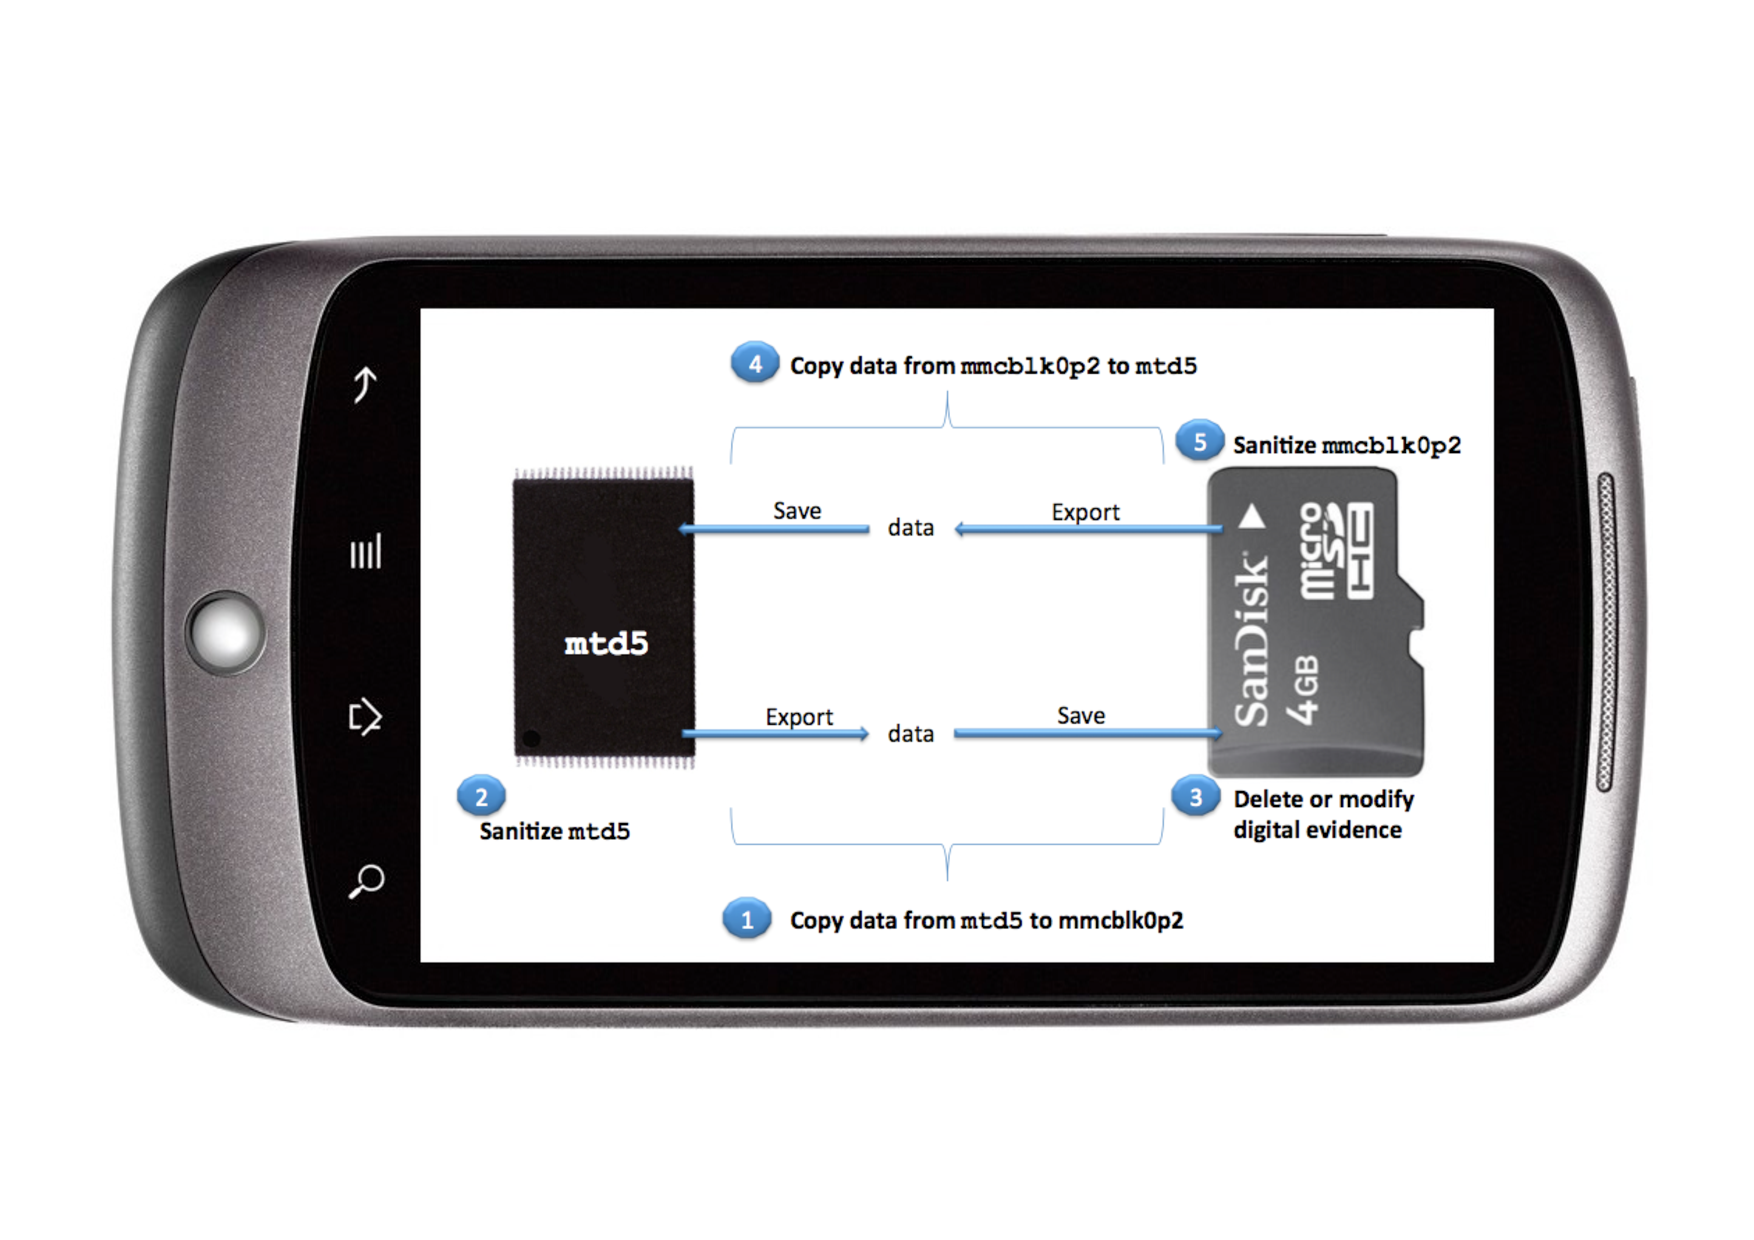
\includegraphics[width=0.84\columnwidth]{figura2.pdf}
\caption{Graphical rappresentation of the proposed technique.}
\label{fig:ProcessoX}
\end{minipage}
\end{figure*}
%    \subsection{ The proposed technique}\label{Method}

\bigskip

The proposed anti-forensics technique has the following three characteristics:
\begin{itemize}
\item The use of only simple software tools which are quite commonly installed on devices running the Android OS. The use of cryptographic techniques and/or kernel modifications would have raised suspicion during a forensics analysis.
%Utilizzo solo di semplici strumenti software preinstallati sul SO Android. L'assenza sia di tecniche crittografiche che modifiche al modulo del kernel che gestisce il file system non genera sospetti in una analisi forense.
\item The deletion is performed in a secure way by overwriting the data. It is also possible to use different sanitization techniques, for example those described in NIST 800-88~\cite{site:NISTGuideLinesSanitization}.
%La cancellazione avviene in modo sicuro sovrascrivendo i dati preesistenti. \`{E} possibile utilizzare tecniche di sanitization a propria scelta, come ad esempio quelle illustrate nel NIST 800-88, Guidelines for Media Sanitization~\cite{site:NISTGuideLinesSanitization}. Con il termine ``sanitization" si indica il processo attraverso il quale si rendono non recuperabili da terzi e ad un'analisi forense i dati presenti su un dispositivo di archiviazione di memoria di massa.
\item The modification is performed without leaving any traces on the device. Moreover, the metadata and attribute list (e.g., timestamp, owner, etc.) can be preserved or changed in a suitable way, so as to not raise any suspicion during a forensics analysis.
%Le modifiche vengono apportate in modo tale da non lasciare alcuna traccia nel sistema. La lista dei metadati e degli attributi (timestamp, owner, etc.) vengono preservati o modificati in modo da non destare sospetti in un'indagine forense.
\end{itemize}

The modification and deletion operations are performed in such a way that any previous copies of the data cannot be recovered or detected.\\

The key idea of the technique is to reduce the selective and secure modification/deletion from a physical level on the NAND to a logical level on the microSD.
The microSD is used as a temporary memorization support. It holds data contained in the internal NAND to allow for its subsequent sanitization. Afterwards, it is possible to selectively delete and modify data on the microSD using logical commands available on the device. Finally, data on the microSD is logically copied back to the internal flash memory. This copy acts only on the allocated files stored on the microSD, ignoring those present on the pages marked as deleted.
%%%%The microSD is used as a temporary memorization support. It holds data contained in the internal NAND to allow the subsequent sanitization of it. Afterwards it is possible to selectively delete and modify data on microSD using logical commands available on the device. Finally, data on microSD is logically copied back to the internal flash memory. This copy acts only on the allocated files stored on the microSD, ignoring those present on pages marked as deleted.
        %La microSD viene utilizzata come supporto di memorizzazione temporaneo destinato ad ospitare i dati contenuti nella %NAND interna al dispositivo e permettere quindi la sanitization di quest'ultima.
        %\`{E} possibile cancellare e modificare selettivamente i dati su microSD utilizzando i comandi disponibili sul SO Android. In seguito alle operazioni di modifica e cancellazione , il contenuto della microSD viene trasferito in flash memory interna utilizzando i comandi prensenti nel SO Android. Questo trasferimento copia tutti i file presenti sulla microSD ignorando quelli allocati su pagine marcate come deleted.

Most of the Android devices collect in the branch \emph{/data} both logs generated by the OS as well as those generated by third-party applications.
However, the file system structure is not the same for all the devices. For example, the Samsung Galaxy S collects these logs in the branch \emph{/dbdata}. Even though the branches of the file system containing such logs are different, they are generally located on the partition \verb"mtd5". Therefore, herein after, the description of the technique will refer to \verb"mtd5" and not to \emph{/data} or \emph{/dbdata}.
After a suitable \emph{Setup} phase, depending on the device and tools used, it is possible to apply the proposed technique.\\

\noindent The technique consists of five steps, as shown in Fig.~\ref{fig:ProcessoX}:

%Ricordiamo che la maggioranza dei dispositivi Android raccolgono nel branch \emph{/data} sia i log generati dal SO, sia quelli generati da applicazioni di terze parti. Bisogna sottolineare che la struttura del file system non \`{e} uguale per tutti i dispositivi. Infatti i dispositivi Android Samsung salvano i log appena citati nel branch \emph{/dbdata}.
%        Nonostante il branch del file system destinato a contenere i log dell'OS e delle applicazioni di terze parti cambi, entrambi sono ospitati nella partizione \verb"/dev/mtd/mtd5".
%        Quindi, nell'illustrazione della tecnica faremo riferimento a \verb"mtd5" e no a \emph{/data} o \emph{/dbdata}.
%
%        Dopo una opportuna fase di \textbf{\emph{Setup}}, che dipende dal dispositivo e dai tool utilizzati, \`{e} possibile applicare la tecnica proposta in questo articolo. Tale tecnica si compone di cinque passi, come illustrato in Figure~\ref{fig:ProcessoX}:
\begin{enumerate}
\item Copy data from \verb"mtd5" to \verb"mmcblk0p2": all the data, including the digital evidence, that has to be deleted or modified are copied to the partition \verb"mmcblk0p2" located on the microSD. The copy is on a logical level.
%tutti i dati, comprese le digital evidence che dovranno essere modificate o concellate, vengono copiati nella partizione \verb"mmcblk0p2" presente sulla microSD. Tale copia avviene a livello logico.
\item Sanitize \verb"mtd5": all the data in the partition \verb"mtd5" is erased using sanitization techniques.
\item Delete or modify digital evidence: the digital evidence, which is located only in \verb"mmcblk0p2", is deleted or modified using logical operations.
%le digital evidence, presenti ormai solo in \verb"mmcblk0p2", vengono modificate o cancellate a livello logico.
\item Copy data from \verb"mmcblk0p2" to \verb"mtd5": all the data, including the digital evidence that has been modified, are copied onto the partition \verb"mtd5".
%il contenuto della partizione \verb"mmcblk0p2" viene ricopiato in \verb"mtd5". Tale copia avviene a livello logico.
\item Sanitize \verb"mmcblk0p2": all the data in the partition \verb"mmcblk0p2" is erased using sanitization techniques.
\end{enumerate}

At the end of the five steps, the partition \verb"mtd5" contains only the data which  were present on the pages marked as allocated on the partition \verb"mmcblk0p2" located on the microSD. In the data, there are the modified files targeted by the anti-forensic modifications. The digital evidence that was logically deleted in step 3) will not be present in the \verb"mtd5" partition since the logical copy operation in step 4) does not copy any of the pages marked as deleted. The partition \verb"mmcblk0p2" will be empty after the five steps. This is not suspicious for the following reasons. Starting from Android v2.2, an application can be installed on the microSD. It is also possible to move a previously installed application from the internal memory to the microSD provided that it has been formatted with the EXT3/EXT4 file system. Therefore, the presence of the partition \verb"mmcblk0p2" does not raise suspicion during a digital forensic analysis. If the device is running an older version of the Android OS, it is preferable to delete such a partition and erase all traces of its existence. The free space resulting from the deletion should be used to expand the partition \verb"mmcblk0p1" to occupy the whole microSD capacity. Clearly, the same operation could be performed even on Android running v2.2 or later, if the user feels that the existence of the partition raises suspicions.

%%%%At the end of the above five steps the partition \verb"mtd5" contains the one and only that data which were present on pages marked as allocated on the partition \verb"mmcblk0p2" located on the microSD. In such data there are the modified files targeted by the anti-forensic modifications. The digital evidence that was logically deleted in step 3) will not be present in the \verb"mtd5" partition since the logical copy operation in step 4) does not copy any page marked as deleted. The partition \verb"mmcblk0p2" will be empty after the five steps. This is not suspicious for the following reason. Starting from Android v2.2, an application ca be installed on the microSD. It is also possible to move a previously installed application from the internal memory to the microSD provided that it has been formatted with the EXT3/EXT4 file system type. Therefore, the presence of the partition \verb"mmcblk0p2" does not raise suspicion in a digital forensic analysis. If the device is running an older version of the Android OS, it is preferable to delete such a partition since it can raise suspicion after a forensics analysis.

%Se la versione di Android presente sul dispositivo mobile \`{e} inferiore alla 2.2 allora, \`{e} consigliato eliminare tale partizione in quanto durante un'analisi forense potrebbe destare non pochi sospetti.

After the application of the proposed technique, there are no pages marked as deleted and containing duplicated blocks in the partitions \verb"mtd5" and \verb"mmcblk0p2".
%%%%After the application of the proposed technique, in the partitions \verb"mtd5" and \verb"mmcblk0p2" there are no pages marked as deleted and containing duplicated blocks. 
Generally, in flash memories there are multiple copies of some blocks. Such a difference could raise suspicions after a forensics analysis. Therefore, it is necessary to artfully produce deleted pages containing duplicated blocks. Since an anomaly detection analysis can distinguish artificial behaviour from real, natural behaviour, it is advisable to generate these pages so that they are similar to the normal Android OS and user behaviour. The content of the \verb"mtd5" partition should be changed to result undistinguishable from a real one by    anomaly detection analysis. However, this analysis is very difficult to perform due to it having to consider both the users behaviour as well as the Android OS functionalities.

%%%%Usually, in flash memories there are multiple copies of some blocks. Such a difference could rise suspicious after a forensics analysis. Hence, it is necessary to artfully produce deleted pages contain duplicated blocks. Since an anomaly detection analysis can distinguish the artful behaviour from the genuine one, it is advisable to generate these pages similarly to the normal Android OS and user behaviour. More generally, the content of the \verb"mtd5" partition should have been changed to result undistinguishable by a anomaly detection analysis from a real one. However, such analysis is very difficult to perform because it should consider both the users behaviour and the Android OS functionalities.
%%%%
Another option that may be used to avoid the detection of the technique by an anomaly detection analysis is to apply some precautions at the beginning of the procedure. In fact, prior to applying the proposed technique, just after having performed a physical acquisition, it would have been collected unallocated pages. These pages should have been verified not being the result of the deletion/modification operations and brought back to their original position in the resulting partition.

%Prima di applicare la nostra tecnica, a seguito di una acquisizione fisica, si potrebbero prelevare pagine non allocate, verificare che non sono duplicazione di quelle relative alla modifica/cancellazione in oggetto, e riportarle nella partizione finale. Chiaramente non sono operazioni a livello logico, ma potrebbero essere pi� semplici dell'analisi menzionata nella versione attuale.
%

%        Dopo l'applicazione della tecnica proposta, in \verb"mtd5" e \verb"mmcblk0p2" non saranno presenti pagine marcate come deleted le quali contengono blocchi duplicati. Si ricorda che normalmente sulle flash memory sono in genere presenti pi\`{u} copie di alcuni blocchi. Questa diversit\`{a} potrebbe creare sospetti a seguito di una analisi forense. Per evitare tali sospetti \`{e} necessario creare artatamente pi\`{u} copie di alcuni blocchi. Per evitare anomaly detection \`{e} importante effettuare tali modifiche in maniera simile al normale comportamento del SO e dell'utente, in modo tale da non lasciare nemmeno il minimo sospetto.
In order to verify the correctness of the proposed technique, a forensic investigation can be carried out by first obtaining the logical and physical acquisitions and then analyzing them, as illustrated in Section~\ref{AndroidForensics}. The analysis includes searching for the digital evidence, which has been deleted by the technique as well as any traces left by the technique itself. An unsuccessful search means a validation of the technique.

%%%%To verify the correctness of the proposed technique one can perform a forensic investigation by first obtaining the logical and physical acquisitions and then analyzing them, as illustrated in Section~\ref{AndroidForensics}. The analysis includes searching for the digital evidence, which has been deleted by the technique. as well as the searching for traces left by the adopted technique itself. An unsuccessful search means a validation of the technique.
%%%%

\section{Case Study}\label{CaseStudy}

The focus of the case study is the application of the proposed technique to a specific device. This case study shows how the technique has been applied, and more generally gives useful advice on its application to different devices.
% The case study is the implementation on a specific device of the technique presented in the above section.
A HTC Nexus One device equipped with the MIUI ROM was been used. The MIUI ROM is a modified Android v2.3.4 by the MIUI Team~\cite{site:MIUI}. With this distribution the user gains root privileges, complete access to the entire file system as well as the possibility to use the BusyBox tool. The BusyBox tool contains all the necessary software modules required for the operations involved in the case study, such as copy, delete, modify, overwrite (i.e., to run the commands \verb=cp=, \verb=rm=, \verb=touch=, \verb=dd=).
%  Si \`{e} utilizzato il dispositivo HTC Nexus One sul quale \`{e} stata installata la MIUI ROM (distribuzione Android 2.3.4 modificata dal team MIUI~\cite{site:MIUI}). Tale distribuzione consente l'accesso completo al file system oltre a fornire il tool BusyBox. Tale tool contiene i moduli software per le operazioni di copia, cancellazione, modifica, sovrascrittura, etc. (e.g. cp, rm, touch, dd, etc.) per applicare la tecnica proposta.
%La presenza del tool BusyBox all'interno del SO Android non desta sospetti in quanto di comune utilizzo.
The  presence of  the BusyBox tool installed on the device does not raise any suspicions since it is quite common to have it installed on an Android device. The structure of the internal flash memory, the microSD as well as the file system on the HTC Nexus One is summarized in Table~\ref{tab:FSTabNexusOne}. The size column shows how big the partitions on the internal flash memory and microSD are.
%%%%
%%%%The presence of the BusyBox tool installed on the device does not rise suspicious since it is quite common to have it installed on an Android device.
%%%% The structure of the internal flash memory, of the microSD and of the file system on the HTC Nexus One is summarized in Table~\ref{tab:FSTabNexusOne}. The size column shows how big are the partitions on the internal flash memory and on the microSD.
%La struttura della flash memory interna, della microSD e del file system presente su tale dispositivo \`{e} riportato in Table~\ref{tab:FSTabNexusOne}. La colonna size riporta la grandezza delle partizioni presenti su flash memory interna e microSD.

\begin{table}
\centering
\begin{tabular}{c|c|c|cp{0.2\columnwidth}}
\hline
\textbf{Partition} & \textbf{Mount Point} & \textbf{Size}\\
\hline
\verb"/dev/mtd/mtd0" & - & - & Internal\\
\verb"/dev/mtd/mtd1" & - & - & Internal\\
\verb"/dev/mtd/mtd2" & - & - & Internal\\
\verb"/dev/mtd/mtd3" & \emph{/system} & 145.0MB & Internal\\
\verb"/dev/mtd/mtd4" & \emph{/cache} & 95.0MB & Internal\\
\verb"/dev/mtd/mtd5" & \emph{/data} & 196.3MB & Internal\\
\hline
\verb"/dev/block/mmcblk0p1" & \emph{/sdcard} & 458.5MB & External\\
\verb"/dev/block/mmcblk0p2" & \emph{/sd-ext} & 3.2GB & External\\
\hline
\end{tabular}
\caption{The structure of the entire file system on the HTC Nexus One running Android v2.2 or later}
\label{tab:FSTabNexusOne}
\end{table}	
                
\subsection{Applying the Technique}

The \emph{Setup} phase includes the following two steps:
\begin{enumerate}
\item The reboot of the device in \emph{recovery mode}. In fact, the copy, delete, modify and overwrite operations cannot be executed while the OS is running.
          %Riavviare il dispositivo in \emph{recovery mode} in quanto le operazioni di copia, cancellazione, modifica e sovrascrittura non sono applicabili mentre il SO \`{e} in esecuzione.
          %\item Verificare il possesso delle credenziali di \emph{root} sul dispositivo.
          %\item Verificare la presenza del tool BusyBox sul dispositivo, in quanto contiene i moduli software per le operazioni di copia, cancellazione, modifica, sovrascrittura, etc. (e.g. cp, rm, touch, dd, etc.) per applicare la tecnica proposta.
          %\item Identificare partizione nel quale vengono salvati i log generati dal SO ed il tipo di file system utilizzato.
\item The verification of the presence of the partition \verb"mmcblk0p2" on the microSD. If this partition is not on the microSD it should be created. This partition has to be empty, with the same file system type of the \verb"mtd5" and not smaller. For example, if the \verb"mtd5" partition has been formatted with the EXT3/EXT4 file system type, then the \verb"mmcblk0p2" partition has to be similarly formatted. The use of the same file system type makes it possible to preserve the metadata and data attribute list during the copy process.
          %Verificare la presenza della partizione \verb"mmcblk0p2" sulla microSD. Se tale partizione non fosse esistita bisognava crearla. Tale partizione deve essere vuota, con lo stesso tipo di file system della partizione \verb"mtd5" e con spazio sufficiente ad ospitare tutti i dati in essa presenti. Se per esempio il tipo di file system presente sul mount point identificato \`{e} di tipo EXT4 allora, la partizione \verb"mmcblk0p2" dovr\`{a} essere presente un file system di tipo EXT4. Utilizzare lo stesso file system permette di non alterare n\'{e} i metadati n\'{e} la lista di attributi dei dati duarante la fase di copia dei dati su microSD.
\end{enumerate}
\medskip

\noindent The description and analysis of the anti-forensics technique for the case study, consisting of the five steps shown in Fig.~\ref{fig:ProcessoX}, is reported below.\\

        %Di seguito viene illustrata l'implementazione e l'analisi dei cinque passi illustrati in Figura~\ref{fig:ProcessoX}.

%\subsubsection*{Copy data from mtd5 to mmcblk0p2}
Copy data from \verb"mtd5" to \verb"mmcblk0p2":
The logical copy of the files from the partition \verb"mtd5" to the partition \verb"mmcblk0p2" has been implemented using the command\\
\begin{footnotesize}
\verb"# mount -o r -t auto /dev/mtd/mtd5 /data"\\
\verb"# mount -o rw -t auto /dev/block/mmcblk0p2 /sd-ext"\\
\verb"# cp -a /data /sd-ext"
\end{footnotesize}

\noindent This command performs the copy by accessing the file system, ignoring the files present on the pages marked as deleted. The parameter \verb"-a" allows for the recursive copy and preservation of the file attribute list (e.g., timestamp, metadata).\\
        %Il comando \verb"cp", presente nel tool BusyBox, utilizzato con i parametri sopra citati consente di copiare in /sd-ext solo i file visibili all'utente e non quelli marcati come deleted, ovvero cancellati. Il parametro ``-a'' permette di copiare in maniera ricorsiva e di preservare la lista degli attributi (timestamp, metadati, etc.) di ogni file oggetto di copia.

%\subsubsection*{Sanitize mtd5}
Sanitize \verb"mtd5":
The secure deletion of the \verb"mtd5" partition is accomplished by overwriting all the pages, without considering whether they are marked allocated or deleted. The overwriting operation consists of setting each bit of the partition to ``0''. Afterwards the partition is formatted in the EXT3/EXT4 file system type. The commands used are the following\\
\begin{footnotesize}
\verb"# dd if=/dev/zero of=/dev/mtd/mtd5 bs=4096"\\
\verb"# mke2fs -T ext4 -b 4096"\\ 
\verb"   -E stride=64, stripe-width=64 -O extent,^huge_file"\\
\verb"   -m 0 -L userdata /dev/mtd/mtd5"
\end{footnotesize}

\noindent It is also possible to use more sophisticated media sanitization techniques, as suggested in~\cite{site:NISTGuideLinesSanitization}, by implementing each overwriting operation with an ad-hoc \verb"dd" command.\\

%\subsubsection*{Delete and modify digital evidence}
Delete and modify digital evidence:
Files on the partition \verb"mmcblk0p2" can be deleted and modified by using the logical functions implemented by the commands of the BusyBox tool. In order to logically delete a file, the command \verb"rm" have been used.
To modify files third-party tools have also been used. For example, using the \verb"MMS.apk", which is a preinstalled application in the Android OS, it is possible to delete a sent or received text message. To modify the timestamp of the database in order to synchronize it with the time of the last SMS present in database, the following command can be used\\
\begin{footnotesize}
\verb"# touch -mt 201101052230.03 mmssms.db"
\end{footnotesize}

\noindent The option \verb"-m" makes it possible to set the last modification time of the database mmssms.db. It is worth mentioning that, in order to make any modifications on the files present in the partition \verb"mmcblk0p2", such partition must be mounted in read-write mode.\\

%\subsubsection*{Copy data from \verb"mmcblk0p2" to \verb"mtd5"}
Copy data from \verb"mmcblk0p2" to \verb"mtd5":
This is the same as the step ``Copy \verb"mtd5" to \verb"mmcblk0p2"'' in which the input and output are exchanged. The command used is\\
\begin{footnotesize}
\verb"# mount -o r -t auto /dev/block/mmcblk0p2 /sd-ext"\\
\verb"# mount -o rw -t auto /dev/mtd/mtd5 /data"\\
\verb"# cp -a /sd-ext /data"\\
\end{footnotesize}

%\subsubsection*{Sanitize \verb"mmcblk0p2"}
Sanitize \verb"mmcblk0p2":
This is the same as the step ``Sanitize \verb"mtd5"'' differing only in the input partition. The commands used are the following\\
\begin{footnotesize}
\verb"# dd if=/dev/zero of=/dev/block/mmcblk0p2 bs=4096"\\
\verb"# mke2fs -T ext4 -b 4096"\\
\verb"   -E stride=64, stripe-width=64 -O extent,^huge_file"\\ 
\verb"   -m 0 -L userdata /dev/block/mmcblk0p2"\\
\end{footnotesize}

\noindent After the five steps, in order to avoid the lack of duplicated pages in the \verb"mtd5" partition, the authors carried out the following operations:
\begin{itemize}
\item send and receive emails;
\item surf on the Internet (this generates many cache files);
\item send and receive SMS;
\item originate some phone calls.
\end{itemize}

Finally, in order to avoid that the partition \verb"mmcblk0p2" would result empty, the authors installed new software on the branch \emph{/sd-ext}.

\subsection{The Technique Validation}
The technique described and implemented in the case study was validated by running multiple experiments, which included many modifications and/or deletions. This was followed by performing both physical and logical acquisitions as well as a forensic analysis on them. During the verification phase, all the open-source tools mentioned in Section~\ref{AndroidForensics}, along with the demo version of Oxygen Forensics Suite 2011, were used.

%%%%The technique described and implemented in the case study was validated by running multiple experiments involving many modifications and/or deletions. Then by performing both physical and logical acquisition and finally a forensic analysis on them. During the verification phase all the open-source tools mentioned in Section~\ref{AndroidForensics} together with the demo version of Oxygen Forensics Suite 2011 have been used.
%In order to test the strength of the case study processes, the capability to acquire the data stored by the internal memory of the device is required.
%we planned to use both commercial tools, general purpose tools and a local application specifically designed to acquire both the data logically and physically stored by the internal memory file system. Among the commercial forensic tools, we selected Oxygen Forensics Suite 2011 that is freely available for demo and testing. Regarding the general purpose tools, we used Nandroid to perform the imaging of the actual device we have.

In order to check the effectiveness of the file deletion operation, several files containing predetermined short patterns were created on the flash memories used. After the application of the technique, the presence of these patterns was searched for. 
The forensic copies of the internal and external flash memories were transferred to an external PC and inspected with a hex-editor so as to perform the search of the patterns. 
In addition, to further test the correctness of the deletion of the digital evidence, digital forensics open-source tools (Autopsy and PhotoREC) were used.
%%%%
%%%%In order to check the effectiveness of the file deletion operation, several files containing predetermined short patterns have been created on the involved flash memories. After the application of the technique, the presence of such patterns has been searched for. To perform the search of the patterns, the forensic copies of the internal and external flash memories have been transferred to an external PC and inspected with an hex-editor. In addition, to further test the correctness of the deletion of the digital evidence, digital forensics open-source tools (Autopsy and PhotoREC) have been used.

In order to validate the anti-forensics technique used to modify files on the device, it was applied to different files several times. All the modifications were carried out on the device without requiring any external hardware. Some modifications were  made  using  the programs  that were shipped with the equipment, while others by using third-party applications. Some of these tools were mentioned in Section~\ref{CaseStudy}. Most of the modifications focused on system applications such as logs, text messages, calls, contacts, emails, etc.. After having applied the modifications, all the files and applications involved were checked to verify whether the changes had been applied or not and the timestamps consistency. Moreover, keeping in mind that flash memories may duplicate some parts of the data, a check was carried out on whether any duplications of the modified information, referring to an unmodified version of it, was found on the device.
%%%%
%%%%In order to validate the anti-forensics technique used to modify files on the device, it has been applied several times on different files. All the modifications have been performed on the device without requiring any external hardware. Some modification were made using programs shipped with the equipment while others by using third-party applications. Some of these tools have been mentioned in Section~\ref{CaseStudy}. Most of the performed modifications have been focused on system applications such as logs, SMS, calls, contacts, emails, etc..
%%%%After having applied the modifications, all the involved files and applications have been checked in order to verify whether the changes have been applied or not and the timestamps consistency. Moreover, keeping in mind that flash memories may keep duplications of some parts of data, it has been checked whether any duplication of the modified information, referring to an unmodified version of it, was found on the device.

All the forensics analysis performed have confirmed the validity of the technique described.
        %
%Inoltre \`{e} stata utilizzata una applicazione di terze parti in grado di effettuare operazioni di file carving dei database contenenti SMS, MMS, chiamate perse e contatti.\\
%
%        Si \`{e} verificata l'esistenza di blocchi duplicati sulle partizioni coinvolte.
        %L'analisi fisica che ha visto coinvolti il tool dd ed un editor esadecimale ha avuto anchessa esito negativo.\\
%        L'immagine fisica non rivela alcun sospetto in quanto le zone di memoria libere sono opportunamente formattate dopo la fase di sanitization.

%    \subsection{Final Results and its Validation}

        %Come descritto nella sezione~\ref{Method}, durante la tecnica proposta le digital evidence vengono modificate o cancellate a livello logico e le partizioni che prima contenevano tali evidence vengono sottoposte ad operazione di sanitization.\\
%        Nel testare la robustezza della tecnica proposta il dispositivo utilizzato \`{e} stato sottoposto ad analisi forense post mortem sia logica che fisica.\\
%        Uno dei possibili strumenti utilizzabili per l'acquisizione logica dei dati ritroviamo Oxygen Forensics Suite 2011.
%        Tale software installa sul dispositivo una applicazione di terze parti in grado di extract le informazioni dai principali database presenti in Android. Tali informazioni vengono salvate in file cvs sulla partizione mmcblk0p1 (branch /sdcard) della microSD. I file frutto di tale acquisizione vengono trasferiti sul PC dove sono analizzati. L'analisi logica, avvenuta come appena illustrato, non ha rilevato le modifiche apportate ai principali database presenti nel SO Android quindi, ha avuto esito negativo.
%        Per l'acquisizione fisica dei dati \`{e} stato utilizzato il tool dd. L'immagine estrapolata con tale tool \`{e} stata poi esaminata con hex editor cercando pattern predeterminati (parte del testo contenuto nei record degli sms cancellati). Tale analisi ha avuto esito negativo, gli unici dati venuti alla luce sono stati quelli presenti sul dispositivo a livello logico.

            %\subsubsection{Experimental workflows}
%
%                In questa sezione si descrive l'experimental workflows della tecnica proposta. L'experimental workflows per tale tecnica \`{e} il seguente:
%                \begin{itemize}
%                  \item Prima immagine logica con il tool Nandroid;
%                  \item Prima immagine fisica della flash memory interna con il tool dd;
%                  \item Applicazione della tecnica proposta;
%                  \item Seconda immagine logica con il tool Nandroid;
%                  \item Seconda immagine fisica della flash memory interna con il tool dd;
%                \end{itemize}
%
%            \subsubsection{Experimental results}
%
%                In questa sezione discuteremo dei risultati ottenuti dalle informazioni acquisite durante gli esperimenti. Il dispositivo incriminato \`{e} stato sottoposto ad analisi forense post-mortem. Abbiamo applicato due tipologie di analisi:
%
%                \begin{itemize}
%                  \item Analisi logica: consiste nell'analizzare il device esplorando il file system dal device stesso. L'esaminatore diventa il comune utilizzatore del dispositivo.
%                  \item Acquisizione ed Analisi della flash memory interna ed esterna: consiste nell'utilizzo di tool di acquisizione logica e fisica della flash memory interna al dispositivo. I dati acquisiti sono poi esaminati da un investigatore forense.
%                \end{itemize}
%
%                Come descritto nella sezione~\ref{Method}, durante la tecnica proposta le evidence vengono modificate o cancellate a livello logico e le partizioni che prima contenevano tali evidence vengono sottoposte ad operazione di sanitization. Dopo l'applicazione di tale tecnica l'analisi logica e fisica del dispositivo mostra la seguente situazione:
%                \begin{itemize}
%                  \item I file cancellati non sono pi\`{u} presenti all'interno del dispositivo.
%                  \item I file modificati non generano sospetti in un'indagine forense, in quanto gli attributi ed i metadati sono stati modificati secondo le proprie esigenze.
%                  \item Il sistema non ha subito alcuna alterazione strutturale, non sono state apportate n\'{e} modifiche al file system, n\'{e} sono state utilizzate tecniche crittografiche.
%                \end{itemize}
%                Per quanto concerne l'analisi logica dei dati acquisiti con il tool Nandroid, \`{e} stato utilizzato il tool unyaffs che ci presenta la struttura del file system acquisito. Tale analisi non ha rilevato alcuna traccia di tecniche anti-forensics.
%                L'analisi fisica che ha visto coinvolti il tool dd ed un editor esadecimale ha avuto anchessa esito negativo.\\
%                L'immagine fisica non rivela alcun sospetto in quanto le zone di memoria libere sono opportunamente formattate dopo la fase di sanitization.
%                Durante gli esperimenti abbiamo risconstrato che \`{e} stata necessaria una solo sovrascrittura bit a bit della partizione \verb"mtd5" affinch\`{e} essa sia opportunamente sanitizzata.


\balance

\section{Conclusions and Future Work}\label{Conclusions}
A new anti-forensics technique for the Android OS was proposed and analyzed. By using the latest digital forensics tools, and considering the specific characteristics of the flash memories used by Android devices, the technique was validated by showing its effectiveness in a case study. 
The technique presented in this work has been used for the construction of a false digital alibi, put forward by De Santis \emph{et al.} in~\cite{alibiprimo}, for the Android OS~\cite{alibiandroid}.


While the device adopted in the case study was a specific mobile phone running the Android OS, the authors plan to investigate their technique further on different kinds of Android device (tablet, smartTV, netbook). 
Moreover, it would be interesting to characterize the distribution of the duplicated pages in order to simulate it as well as pass any eventual anomaly detection inspections.

Finally, considering that the type of memories used by the majority of the Android devices are the same as those used by most mobile devices, a future study could be carried out on devices using similar types of memories (e.g., Apple iPhone).


%%%%A new anti-forensics technique for the Android OS has been proposed and analyzed. By using the latest digital forensics tools, and considering the specific characteristic of the flash memories used by the Android devices, the technique has been validated showing its effectiveness in a case study. Whereas in the case study the device adopted has been a specific mobile phone running the Android OS, the authors plan to further investigate their technique even on different kind of Android devices (tablet, TV, netbook). Moreover, considering that the type of memories used by the majority of the Android devices are the same used by most of all the other mobile devices, a future study could be performed on devices using similar types of memories (e.g., the Apple iPhone).
%%%%
%%%%It could be interesting to characterize the distribution of the duplicated pages in order to simulate it and survive to any eventual anomaly detection inspection. 
    
    %A more detailed study on the algorithm , which should considers how the flash memories store and duplicate data without user awareness, should be performed in order to make the results of the presented anti-forensics technique as close as to the behaviour of the flash memory controllers. Knowing that behaviour it is important to refine the testing phase of the technique which will check the unwanted duplicated data to be coherent with the normal functioning of the flash memory technology.

    %Uno studio pi� approfondito su come Android duplica i dati sul supporto di memorizzazione all'insaputa dell'utente dovrebbe essere effettuato in modo tale da far si che le tecniche di anti-forensic presentate nel lavoro lascino i dati duplicati in maniera simile a come normalmente Android fa.

    %A more detailed study which considers the anomaly detection matter could be investigated in order to make

%To avoid suspects it is necessary to produce deleted pages contain duplicated blocks. To avoid suspects even in the case of a anomaly detection analysis it is necessary to generate these pages similarly to the SO and user behaviour.

%In questo articolo abbiamo proposto una nuova tecnica Anti-Forensic per i dispositivi mobile Android, l'abbiamo %implementata in un caso di studio reale e l'analisi forense ha confermato la sua validit\`{a}.

%Verificare la possibilit\`{a} di implementare il tutto anche su dispositivi Android diversi e su sistemi operativi diversi (iPhone) perch\`{e} la tecnologia utilizzata \`{e} simile. Una possibile estensione del lavoro pu\`{o} essere quella di testare la tecnica considerando la questione Anomaly Detection facendo una classificazione preliminare del comportamento su Android.

%Lista delle figure
%\clearpage
%\listoffigures
%lista delle tabelle
%\listoftables
%Bibliografia

\bibliographystyle{IEEEtran}
\bibliography{android}

%\bibliographystyle{alpha}
%\bibliography{AndroidAntiForensicsdata2SD}

\end{document} 